\documentclass{article}
\usepackage{amsmath}
\usepackage{color}
\usepackage{graphicx}
%\usepackage{hyperref}

\renewcommand{\thesection}{\arabic{section}.}
\renewcommand{\thesubsection}{(\alph{subsection})}

\pagestyle{empty}
%\hypersetup{colorlinks=true, linkcolor=blue}

\begin{document}
\section{}
The model is
\begin{align}
    Y &= C(Y - T) + I(r) + G + X(e, Y), \label{eq1}\\
    \frac{M}{P} &= L(r, Y), \label{eq2}\\
    X(e, Y) &= F(r). \label{eq3}
\end{align}
Plug \eqref{eq3} into \eqref{eq1} and together with \eqref{eq2} we can get two curves with respect to $r$ and $Y$.
For the equation \eqref{eq1}, i.e. the IS equation,
\[
    \frac{\partial r}{\partial Y}
    = -\frac{C' - 1}{I' + F'} < 0,
\]
For the equation \eqref{eq2}, i.e. the LM equation, 
\[
    \frac{\partial r}{\partial Y}
    = -\frac{L_2}{L_1} > 0,
\]
in which $L_1 \equiv \partial L / \partial r$, $L_2 \equiv \partial L / \partial Y$. Therefore, we get a downward-sloping IS curve and an up-sloping LM curve, whose intersection determines the equilibrium state $(r^\ast, Y^\ast)$. Then we can find the exchange rate in the equilibrium through \eqref{eq3}.

When there is a decline in investment sentiment, which implies for every $r$, $I(r)$ decreases, the IS curve shifts to the left. This results in both lower output and interest rate. And a lower $r^\ast$ means a higher $F(r^\ast)$. To satisfy \eqref{eq3}, $X$ must be higher. With $\partial X / \partial Y < 0$ and $\partial X / \partial e < 0$, we can not conclude how the exchange rate changes.

\section{}
\subsection{}
Plug in all the expressions into the IS and LM equation:
\[
    \begin{cases}
        Y = a + b \cdot (Y - T) + d - e \cdot r + G \\
        \dfrac{M}{P} = M_0 + f \cdot Y - g \cdot r
    \end{cases}
\]
Eliminating $r$, we then get the AD curve:
\[
    e \left(M_0 + f \cdot Y - \frac{M}{P}\right)
    = g (a + d + G - Y) + g \cdot b  (Y - T).
\]

\subsection{}
When there is a negative shock to the investment sentiment, the AD curve becomes
\[
    e \cdot \frac{M}{P} = \left(g (1 - b) + e \cdot f\right) Y + e \cdot M_0 - g(a + d - d_0 + G - b \cdot T)
\]
which shows a decline in the intercept. Meanwhile,
\[
    \frac{\partial P}{\partial Y}
    = -\frac{e \cdot f + g - g \cdot b}{e \cdot M} \cdot P^2 < 0,
\]
which means that the AD curve is downward-sloping. Therefore, the AD curve shifts to the left by $d_0 \cdot g / (g(1-b) + e\cdot f)$.

\section{}
\subsection{}
The model is
\begin{align}
    Y &= C(Y - T) + I(r^\ast) + G + X(e),\notag \\
    \frac{M}{P} &= L(r^\ast, Y).\label{eq4}
\end{align}
Note that $P$ is only subject to equation \eqref{eq4}. Therefore, the AD equation is actually the LM equation with an accepted $r^\ast$.
\begin{figure*}[h]
    \centering
    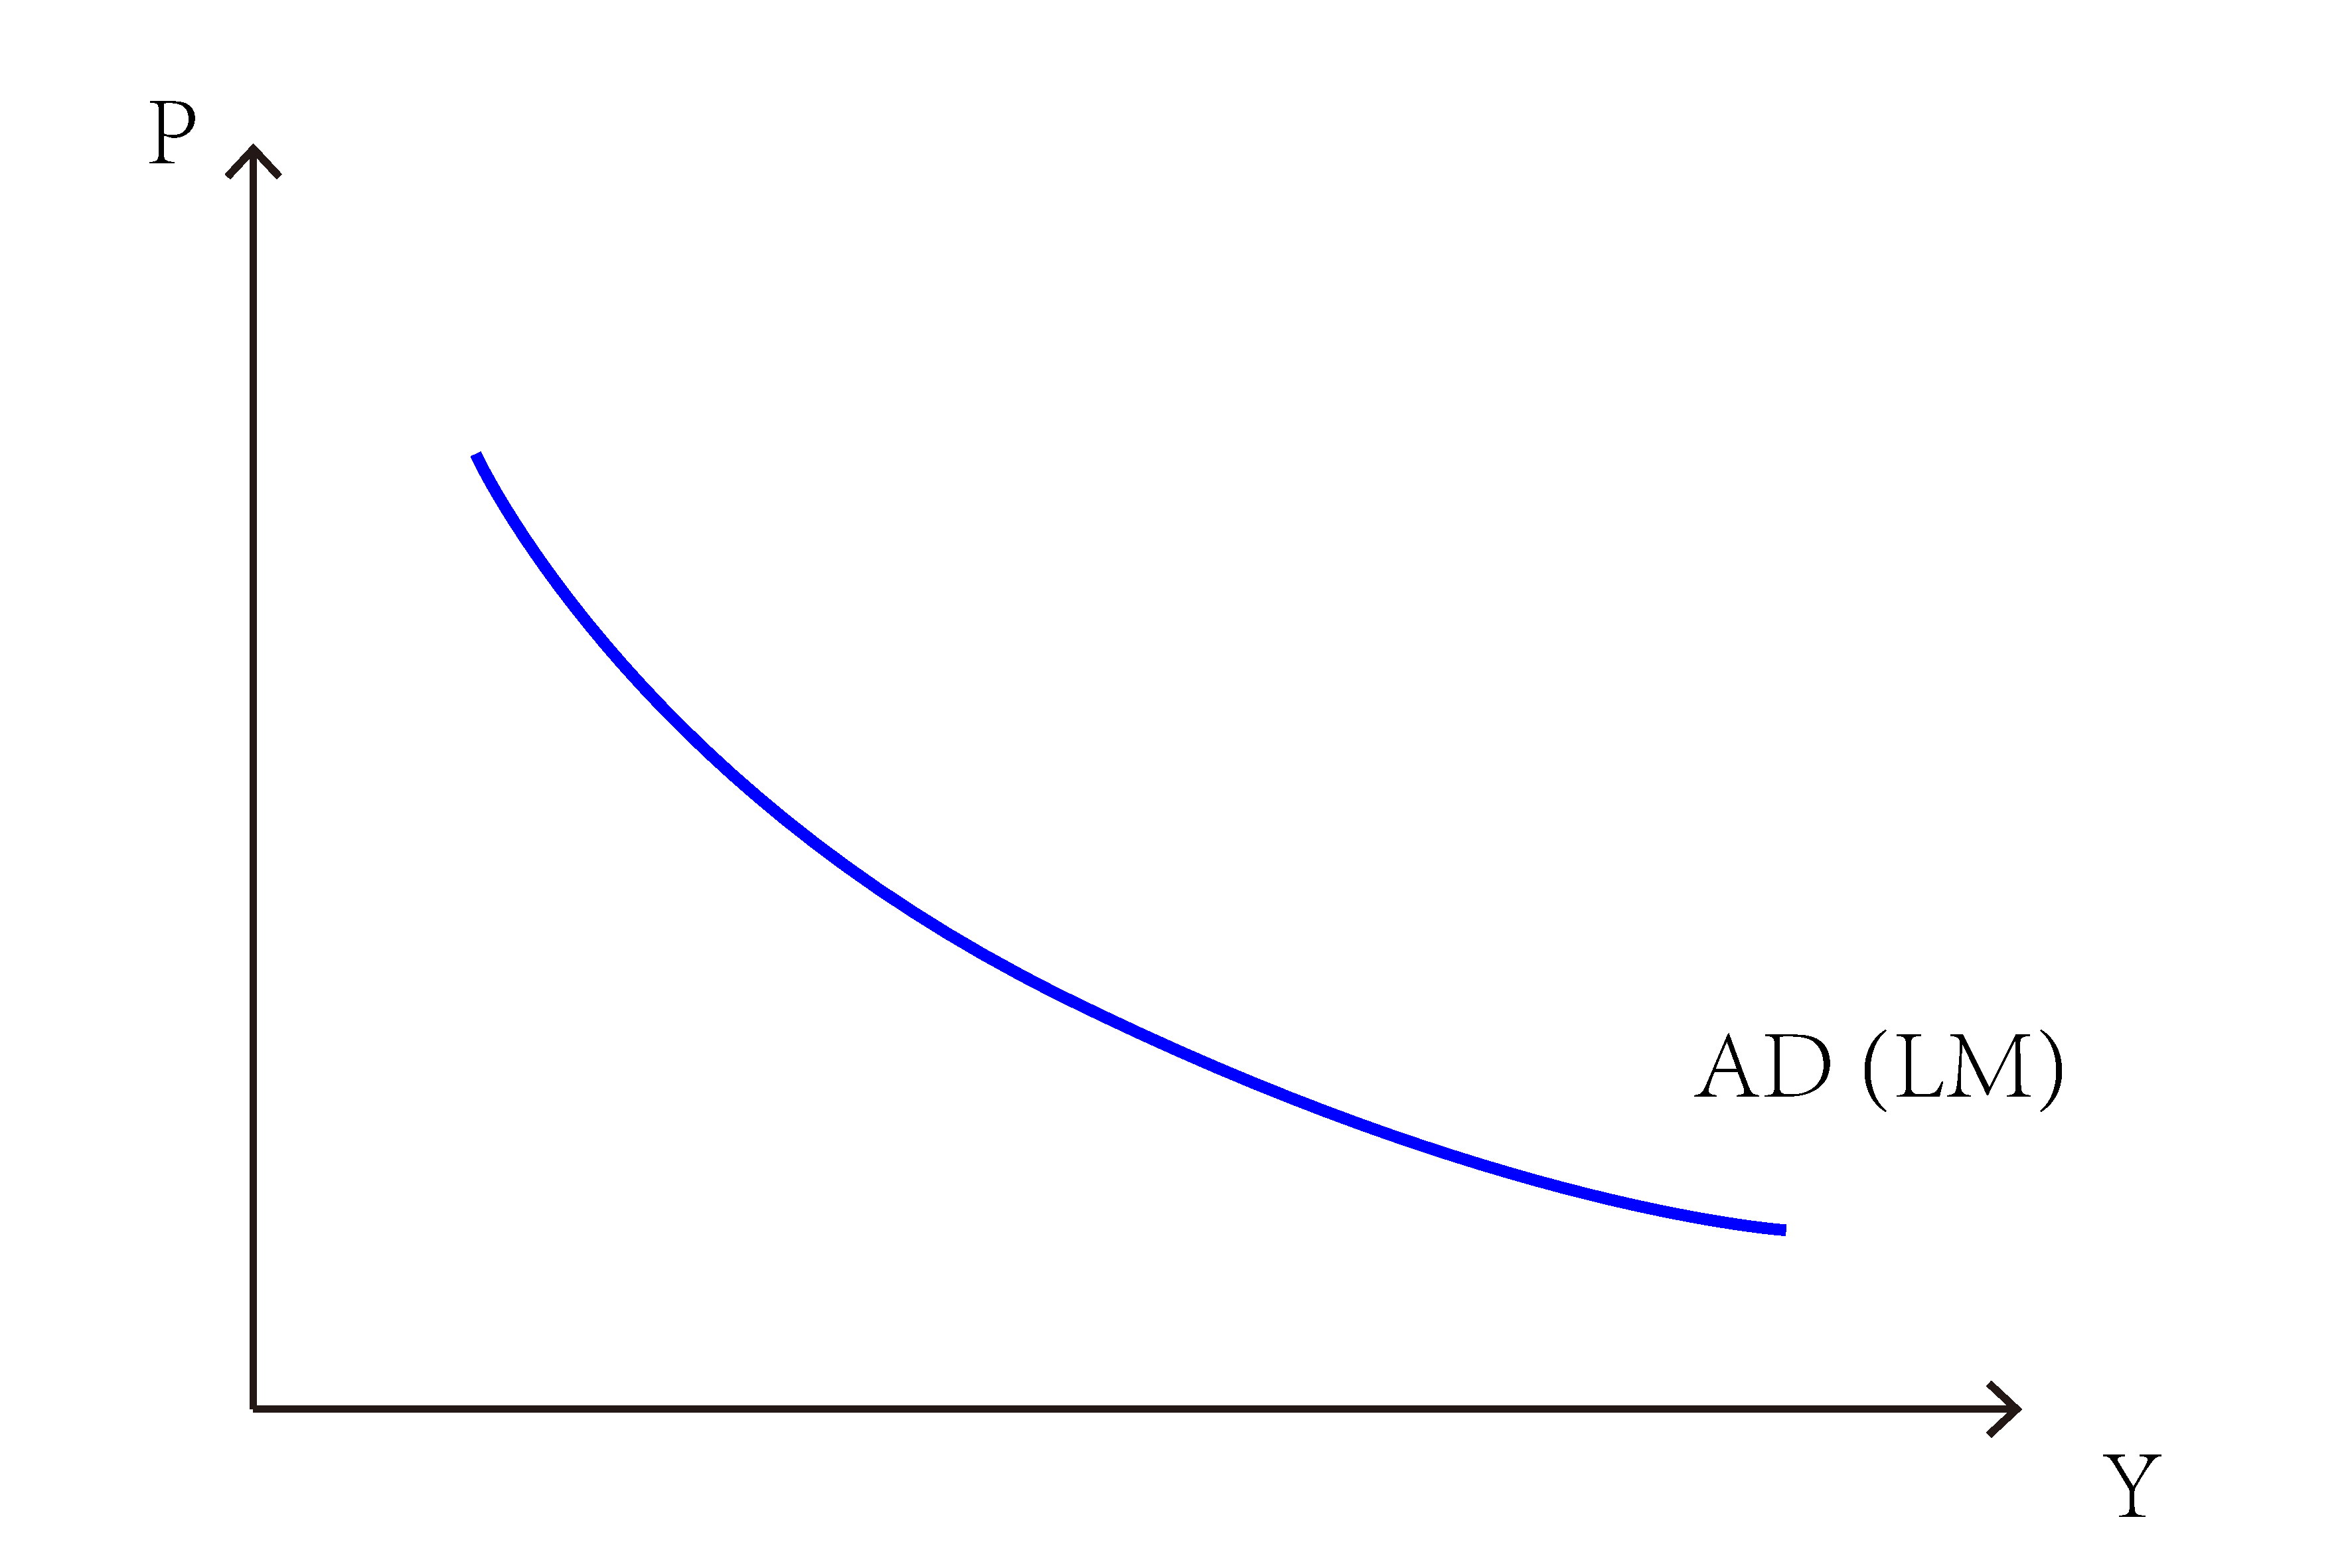
\includegraphics[scale=0.15]{figure/3-1.pdf}
\end{figure*}

\subsection{}
The model is
\begin{align}
    Y &= C(Y - T) + I(r^\ast) + G + X(e^\ast),\label{eq5} \\
    \frac{M}{P} &= L(r^\ast, Y).\label{eq6}
\end{align}
Note that in equation \eqref{eq5}, $Y$ is determined, which implies $L$ is also determined in \eqref{eq6}. $P$ and $M$ adjust to satisfy equation \eqref{eq6}. Therefore, the AD curve is a straight line.
\begin{figure*}[h]
    \centering
    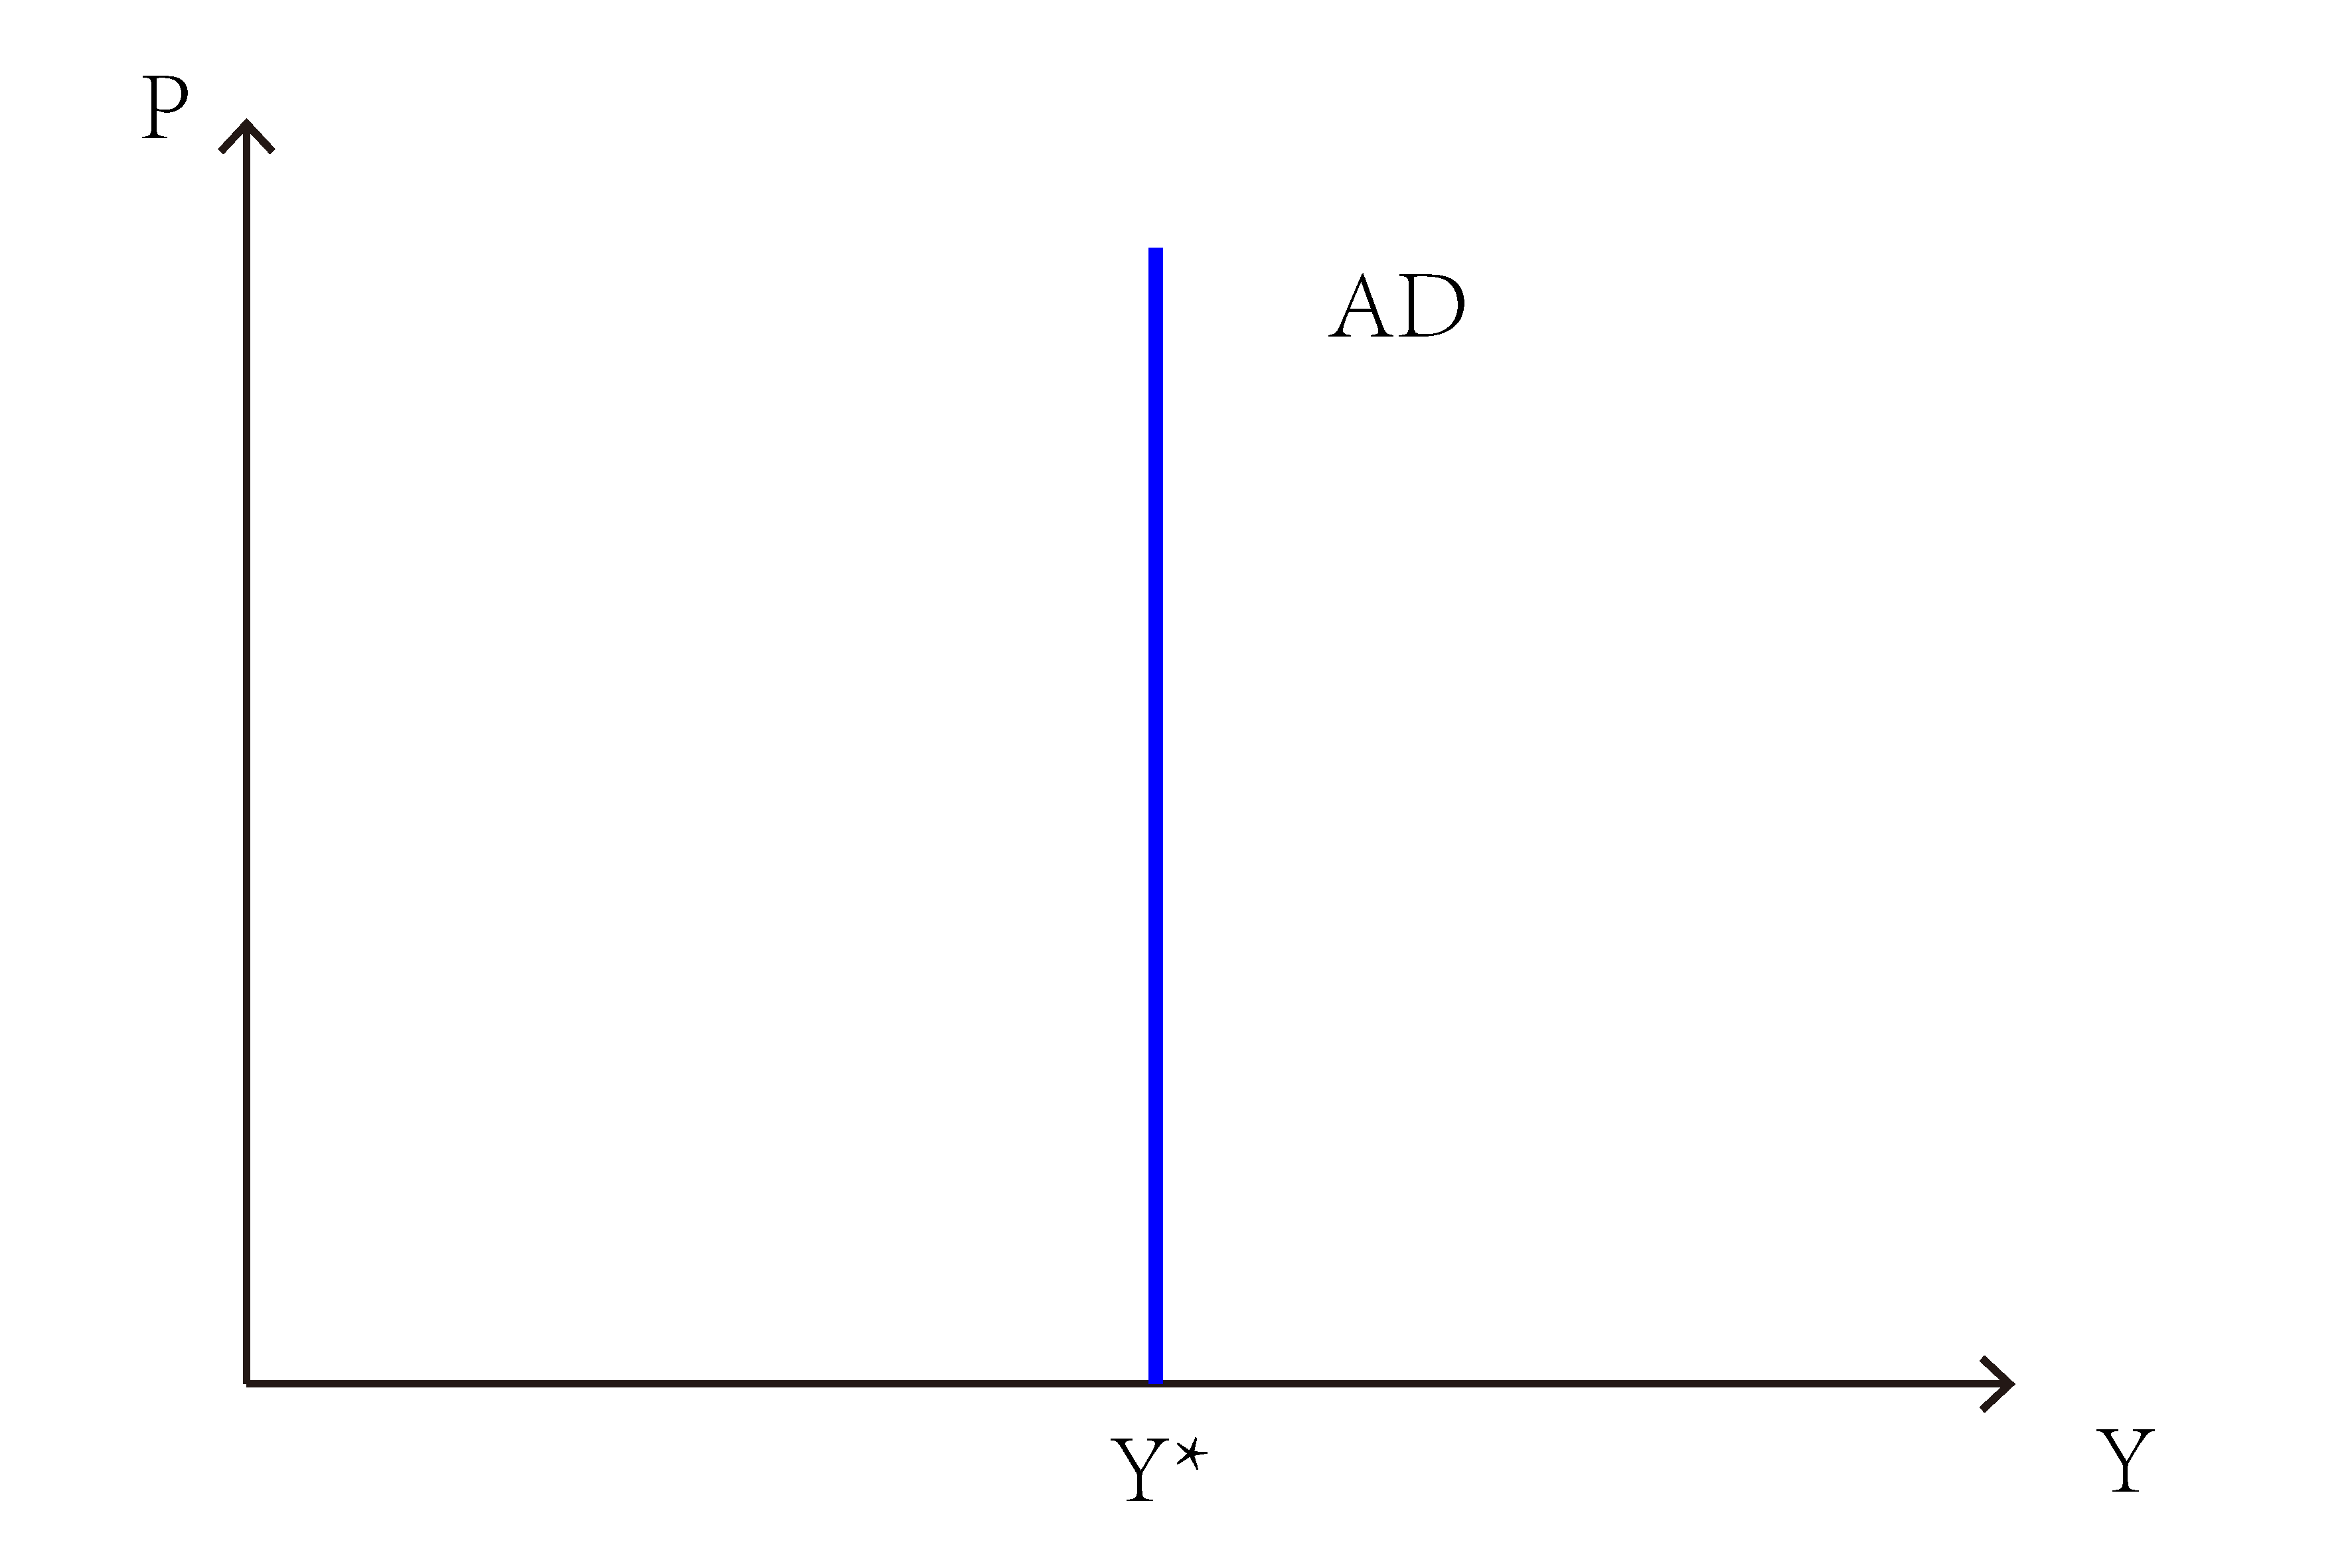
\includegraphics[scale=0.15]{figure/3-2.pdf}
\end{figure*}
\end{document}